\chapter{静电场}
\section{电荷守恒定律}
\subsection{电荷量}
电荷的多少叫做电荷量(electric quantity).它是一个标量,单位是: 库仑(coulomb)符号为:$C$.
\subsection{电荷的量子化---元电荷}
实验证实所有的电荷量都是 $1.6\times 10^{-19}C$ 的整数倍,我们记此电荷量为 $e=1.6\times 10^{-19}C$ 称作\CJKunderwave{原电荷}\footnote{
原电核的数值最早由美国物理学家\CJKunderwave{密立根}(R.A.Millikan,1868-1953) 使用 \CJKunderwave{油滴实验} 测定.
}(elementary charge).

\subsection{比荷}
 在电学的计算中,分析电荷的加速偏转等问题时经常需要计算粒子的加速度等,所以这里就引入一个物理量---比荷,即带电粒子电荷量与其质量的比值.例如电子的比荷为:

 \begin{equation}
   \cfrac{e}{m_e}=1.76\times 10^{11}C/kg
 \end{equation}

 \subsection{三种起电方式}
 \subsubsection{摩擦起电}

 物体由原子构成,原子又由原子核与核外电子构成,在物体的表面充满了电子云.当两个\CJKunderwave{不同的物体}相互接触且发生挤压时,这此电子云就会相互排斥而分开,在挤压的这个点上就暴露出了一些正电荷,则当相互分开(摩擦)时,对电子吸引能力强的原子核将会获得更多的电子而带负电,对电子吸引能力弱一点的原子核就会带正电.一般同种物质相互摩擦时也可以因摩擦而带电,但是二者对电子的吸引能力相当,则因此而使物体所带的电荷量很少,所以一般使用不同的绝缘的物体相互摩擦起电.

 \subsubsection{感应起电}

当一个已经带电的物体靠近一个金属导体或者溶液时,会由于同种电荷相互排斥异种电荷相互吸引而使靠近此物体的金属或溶液的一端带异种电荷,远离此物体的一端带同种电荷.这时,如果不移开带电体,而使金属或溶液从中间一分为二,则这二部分将分别带正电和负电,且电荷量相等.这就是感应起电.

\subsubsection{接触起电}

当使用一个带电的导体接触另一个不带电的导体时电荷就会在这二者之间重新分配,如果两个导体同时都带电,则它们的电荷将会先中和然后再分配.如果两个物体是完全相同的物体,则电荷在它们之间先中和再平分.

在高中物理中经常遇到三个全同金属小球相互接触计算最后所带电量的题目,这里经过分析我提出一种非常有条理的书写方法.

\begin{calculate}
1.以三个小球A,B,C 分别带电$8C$ , $-6C$, $0$ ,并且先让C与A接触,再让C与B接触,问最后各小球的带电量是多少?

e.如下图所示书写步骤

\end{calculate}

\begin{figure}[H]
  \centering
  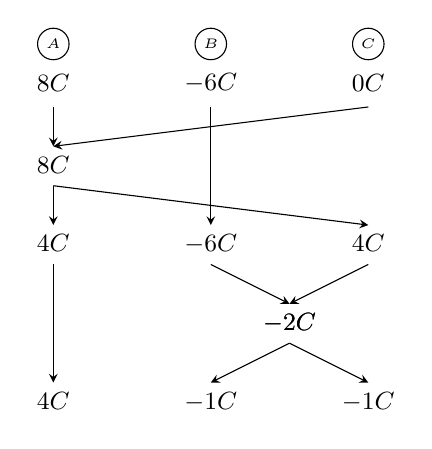
\begin{tikzpicture}
    \draw (-2,0) node {\tiny $A$} circle [radius=0.2]; 
    \draw (0,0) node {\tiny $B$}circle [radius=0.2]; 
    \draw (2,0) node {\tiny $C$}circle [radius=0.2]; 
    \draw (-2,-0.5) node {\small $8C$};
    \draw (0,-0.5) node {\small $-6C$};
    \draw (2,-0.5) node {\small $0C$};
    \draw [->,>=stealth] (-2,-0.8) -- (-2,-1.3);
    \draw [->,>=stealth] (2,-0.8)--(-2,-1.3) node [anchor=north] {\small $8C$};
    \draw [->,>=stealth] (-2,-1.8) -- (-2,-2.3) node [anchor=north] {\small $4C$};
    \draw [->,>=stealth] (-2,-1.8)--(2,-2.3) node [anchor=north] {\small $4C$};
    \draw [->,>=stealth] (0,-0.8) --(0,-2.3) node [anchor=north] {\small $-6C$};
    \draw [->,>=stealth] (0,-2.8) -- (1,-3.3) node [anchor=north] {\small $-2C$};
    \draw [->,>=stealth] (2,-2.8) -- (1,-3.3) node [anchor=north] {\small $-2C$};
    \draw [->,>=stealth]  (1,-3.8)-- (0,-4.3) node [anchor=north] {\small $-1C$};
    \draw [->,>=stealth]  (1,-3.8)-- (2,-4.3) node [anchor=north] {\small $-1C$};
    \draw [->,>=stealth] (-2,-2.8)--(-2,-4.3) node [anchor=north] {\small $4C$};
  \end{tikzpicture}
  \caption{接触起电的计算}
  \label{fig:jiechuqidian}
\end{figure}

注意:这个书写方式的具体实现是,先把三个待处理的带电小球并排一行,然后在其下面标上电荷数,第一次 $C$ 与$A$ 接触,则画箭头到 $A$ 的正文,并写上它们中和后的电量 $8C$ ,然后再画箭头到各自下面写出平分后的电荷.$B$没有参与电荷的分配,则用箭头直接往下画到与上一步同一高度的一行,再令$B$和 $C$ 分别画箭头到 $B$
和$C$ 之间的下方写出它们中和后的电荷量,然后再用箭头画回到各自下方,标出平分后的电荷量 $1C$.最后将此次没有参考电荷分配的 $A$ 直接用箭头画到同一高度处,则经过处理后三个带电小球的电荷量就依次排开了,分别为$4C$,$-1C$,$-1C$.


\subsection{电荷守恒定律}

\subsubsection{电荷守恒定律的经典表述}

电荷即不会创生,也不会消灭,它只能从一个物体转移到另一个物体,或者从一个物体转移到另一个物体:在转移过程中,电荷的总量保持不变.此结论叫做电荷守恒定律(law of conservation of electric charge).

\subsubsection{电荷守恒定律的现代表述}

\CJKunderwave{
一个与外界没有电荷交换的系统,电荷的代数和保持不变.
}

近代的物理实验表明,在一定的条件下,带电粒子可以产生和湮灭.例如:一个高能光子可以产生一个正电子\footnote{正电子与电子质量相同,与电子的电荷量相等但符号相反.于1932年发现}和一个负电子;一对正、负电子可以同时湮没,转化为光子.但是,带电粒子的产生和江油总是成对的,两个带电粒子电荷数量相等但是正负相反,而光子不带电,所以在此系统与外界没有电荷交换的前提下电荷的代数和仍然不变.电荷守恒定律是自然界最重要的基本规律之一.

\section{库仑定律(Coulomb law)}
\subsection{点电荷(electrostatic force)}

当带电体间的距离比它们自身的大小大得多,以至于带电体的形状、大小及电荷分布状况对它们之间的作用力的影响可以忽略时,这样的带电体就可以看做带电的点,叫做点电荷\footnote{点电荷类似于力学中的质点,也是一种理想化的物理模型}(point charge).

\subsection{库仑定律}

\subsubsection{内容}
\CJKunderwave{真空中}两个\CJKunderwave{静止点电荷}之间的相互作用力与它们的电荷量的乘积成正比,与它们的距离的二次方成反比,作用力的方向在它们的连线上.电荷间的这种相互作用力叫做静电力(electrostatic force) 或库仑力.

\subsubsection{表达式}

\begin{equation}
  F=k\cfrac{q_1q_2}{r^2}
  \label{eq:coulomblaw}
\end{equation}

\subsubsection{对公式的解释}

式\eqref{eq:coulomblaw} 中的 $k$ 是比例系数,叫做静电力常量(electrostatic force constant) .在国际单位制中,电荷量的单位是库仑($C$),力的单位是牛顿($N$),距离的单位是米($m$),则 $k$ 的数值由实验测定为

\begin{equation}
  k=9.0\times 10^9 N\cdot m^2/C^2
  \label{eq:coulombconst}
\end{equation}

在使用库仑定律\eqref{eq:coulomblaw} 时,对于电荷量有两种处理方案.其一:$q_1$ 和 $q_2$ 都不带正负号,在判断方向时,根据同号相斥异号相反来判断.其二:$q_1$ 和$q_2$ 都带上正负号,这和后面的能量部分是统一的.如图\ref{fig:coulombdirection}所示,如果计算 $q_2$ 所受到的库仑力,则选图中箭头所示的方向为正,显然如果两个点电荷同号则 $F>0$ 为斥力,如果两个点电荷异号则 $F<0$ 为引力.

\begin{figure}[H]
  \centering
  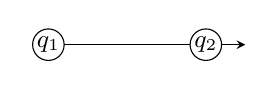
\begin{tikzpicture}
    \draw (-1,0) node {\small $q_1$} circle [radius=0.2]; 
    \draw (1,0) node {\small $q_2$} circle [radius=0.2]; 
    \draw (-0.8,0)--(0.8,0);
    \draw [->,>=stealth] (1.2,0)--(1.5,0);
  \end{tikzpicture}
  \caption{库仑定律的方向}
  \label{fig:coulombdirection}
\end{figure}

\section{电场强度}
\subsection{超距作用}

万有引力曾经被认为一种即不需要媒介,也不需要经历时间,而是超越空间和时间直接发生的作用力,被称为超距作用.

\subsection{电磁场(electromagnetic field)}

电场是一种客观存在的物质,这在不同的情况下表现为不同的形式,如果电荷运动起来则表现出磁性,也就是磁场和电场是同一种物质的不同表现形式,统称为电磁场(electromagnetic).变化的电磁场可以以光速传播,且与机械波不同,电磁场传播不需要介质.

举个例子来类比说明电磁场.例如,化学上大家学过 $H_2O$ ,这是水的化学式,也可以认为是一种物质,在零上它表现为液态,在零下表现为固态.显然水和冰在本质上是同一种物质,但是不同情况下表现出不同的物理特征.所以电磁场也是如此,有的情况下表现为电场有的时候表现为磁场.

\subsection{电场强度(electic field strength)}

\subsubsection{静电场}

对电磁场的介绍我们是按照由特别到一般的顺序进行,所以我们先介绍一种特殊情况,\CJKunderwave{静止电荷产生的电场},称为静电场(electrostatic field).

\subsubsection{电场的特征}

电场的特征之一是对放入电场中的电荷有力的作用.

\subsubsection{电荷的量子化}

在前方中已经提到电荷量总是元电荷的整数倍,这称为电荷的量子化.

\subsubsection{电场强度}

结合电场对电荷具有力的作用和电荷的量子化,我们能够推断,在电场中若放入一个试探电荷
\footnote{试探电荷是用来测试电场的电荷,它的电荷量不能太大因为它自身也有电场,它不能干扰要测定的电场,同时为了确保测量的精度它的体积也不能太大.试探电荷可以有正负}
则它要受到电场力的作用,由于电荷量总是元电荷的整数倍,所以这等效于放入了$\frac{q}{e}$ 个元电荷所受到的力,因此我们可以得到试探电荷$q$ 所受到的电场力正比于等效元电荷的数目,也就是

\[
  F\propto n=\cfrac{q}{e}
\]

上式也表明,这个力正比于试探电荷的电荷量,定义这个比值为电场强度.同时不同的地方试探电荷所受力的方向也不相同,因此这个比值所定义的物理量电场强度是一个矢量,规定\CJKunderwave{正的试探电荷}所受电场力的方向是电场强度的方向.定义式为

\begin{equation}
  E=\cfrac{F}{q}
  \label{eq:ElecticFieldStrength}
\end{equation}


按照式 \eqref{eq:ElecticFieldStrength} 可得,电场强度的单位是{\bf 牛[顿]每库[仑]},符号为 $N/C$. 由于在后面我们还要讨论到电场强度和电势差的关系
\footnote{电场强度与电势差的关系:$U=Ed$}
,所以它还有另一个单位{\bf 伏[特]每米}, 符号是$V/m$,这两个单位是等价的,即$1V/m=1N/C$.

\subsubsection{点电荷的电场强度}

点电荷是最简单的场源电荷,前面已经介绍了真空中两个点电荷间的相互作用力---库仑力.设一个点电荷的电荷量为 $Q$,与之相距$r$的试探电荷的电荷量为$q$,据库仑定律和电场强度的定义得

\begin{equation}
  \left.
  \begin{gathered}
    F=k\cfrac{Qq}{r^2}\\
    E=\cfrac{F}{q}
  \end{gathered}
\right \}
\Longrightarrow
E=k\frac{Q}{r^2}
  \label{eq:EFSpoint}
\end{equation}

可以证明
\footnote{由于同学位目前数学水平所限不能详细证明,在大家上了大学之后在\CJKunderwave{电动力学}课程中会有相关证明}
,上述公式不仅适用于真空中的点电荷,也适用于电荷均匀分布的球,但是式中$r$是指空间中的一点到球心的距离.

\begin{figure}[H]
  \centering
  \begin{tikzpicture}
    \draw (0,0) node {\small $+$} circle [radius=0.3];
    \draw [dotted] (0,0) circle [radius=1];
    \draw[->,>=stealth] (0:1)--(0:1.5);
    \draw[->,>=stealth] (45:1)--(45:1.5);
    \draw[->,>=stealth] (90:1)--(90:1.5);
    \draw[->,>=stealth] (135:1)--(135:1.5);
    \draw[->,>=stealth] (180:1)--(180:1.5);
    \draw[->,>=stealth] (225:1)--(225:1.5);
    \draw[->,>=stealth] (270:1)--(270:1.5);
    \draw[->,>=stealth] (315:1)--(315:1.5);
    \draw (0,-1.5) node [anchor=north] {\small 正电荷};
  \end{tikzpicture}
  \qquad
  \begin{tikzpicture}
    \draw (0,0) node {\small $+$} circle [radius=0.3];
    \draw [dotted] (0,0) circle [radius=1.5];
    \draw[->,>=stealth] (0:1.5)--(0:1);
    \draw[->,>=stealth] (45:1.5)--(45:1);
    \draw[->,>=stealth] (90:1.5)--(90:1);
    \draw[->,>=stealth] (135:1.5)--(135:1);
    \draw[->,>=stealth] (180:1.5)--(180:1);
    \draw[->,>=stealth] (225:1.5)--(225:1);
    \draw[->,>=stealth] (270:1.5)--(270:1);
    \draw[->,>=stealth] (315:1.5)--(315:1);
    \draw (0,-1.5) node [anchor=north] {\small 负电荷};
  \end{tikzpicture}
  \caption{点电荷的电场}
  \label{fig:EFSpoint}
\end{figure}

\subsubsection{电场线}

使用公式描述电场比较精确,但是不够形象,法拉第采用了一个简洁的方法描述电场,它不能给出具体值,但是能够方便的判断场强的相对大小和方向,这就是电场线.电场线具备一些特点,下面具体讨论.

\begin{enumerate}
  \item 电场线起于正电止于负电,是不闭合的曲线(有的书上说起于无穷远或止于无穷远,是因为在无穷远处有正电荷或负电荷).
  \item 电场线的疏密表示场强的大小.
  \item 电场线的切线方向表示场强的方向.
  \item 电场线不能相交(因为空间中一点场强只能有一个方向,如果相交则该点将不能确定场强的具体方向).
  \item 电场线不能相切(这一点大家注意,它并不违反场强方向唯一性,但是由于疏密程序表示大小,所以相切即无穷密,则场强无穷大,这在物理上也是不合理的).
\end{enumerate}
\begin{figure}[H]
  \centering
  \begin{tikzpicture}
    \draw[->,>=stealth] (0,0) arc (180:90:1.5);
    \draw[->,>=stealth] (1.5,0) arc (0:90:1.5);
    \draw (60:1.5) circle [radius=1pt] node [anchor=north]{\small P};
    \draw [->,>=stealth] (60:1.5)--++(30:0.6) node [anchor=west]{\tiny E};
    \draw [->,>=stealth] (60:1.5)--++(150:0.6) node [anchor=east]{\tiny E};
    \draw (60:1.5) node [anchor=south]{\small ?};
    \draw (0.75,-0.5) node {\small 电场线不相交};
  \end{tikzpicture}
  \qquad
  \begin{tikzpicture}
    \draw[->,>=stealth] (0,0) arc (180:90:1.5);
    \draw[->,>=stealth] (1.5,0)++(135:3)++(0,-1.5) arc (270:360:1.5);
    \draw[->,>=stealth] (1.5,0)++(135:1.5)--++(45:0.8) node [anchor=south west]{\tiny E};
    \filldraw (1.5,0)++(135:1.5) circle [radius=1pt] node [anchor=north]{\tiny P};
    \draw (0.75,-0.5) node {\small 电场线不相切};
  \end{tikzpicture}
  \caption{电场线的性质}
  \label{fig:dianchangxian}
\end{figure}

\subsubsection{六种常见的电场线}

%\begin{figure}[H]
%  \centering
%  \begin{tikzpicture}
%    \draw (-2,0) circle [radius=0.2] node {\small $+$};
%    \draw (2,0) circle [radius=0.2] node {\small $-$};
%   \draw (-1.8,0.2) parabola bend (0,0.5) (1.8,0.2); 
%   \draw (-1.9,0.3) parabola bend (0,1.3) (1.9,0.3); 
%   \draw (-2,0.3) parabola bend (0,2.3) (2,0.3); 
%   \draw (-1.8,0)--(1.8,0);
%   \draw (-1.8,-0.2) parabola bend (0,-0.5) (1.8,-0.2); 
%   \draw (-1.9,-0.3) parabola bend (0,-1.3) (1.9,-0.3); 
%   \draw (-2,-0.3) parabola bend (0,-2.3) (2,-0.3); 
%   \draw[->,>=stealth] (-0.1,2.3)--(0.1,2.3);
%   \draw[->,>=stealth] (-0.1,1.3)--(0.1,1.3);
%   \draw[->,>=stealth] (-0.1,0.5)--(0.1,0.5);
%   \draw[->,>=stealth] (-0.1,0)--(0.1,0);
%   \draw[->,>=stealth] (-0.1,-0.5)--(0.1,-0.5);
%   \draw[->,>=stealth] (-0.1,-1.3)--(0.1,-1.3);
%   \draw[->,>=stealth] (-0.1,-2.3)--(0.1,-2.3);
%   \draw(-2.3,0)--(-3.3,0);
%   \draw[->,>=stealth] (-2.5,0)--(-2.7,0);
%   \draw(2.3,0)--(3.3,0);
%   \draw[->,>=stealth] (2.7,0)--(2.5,0);
%   \draw [->,>=stealth](-2.3,0.2) arc (220:180:2);
%   \draw [->,>=stealth](-2.3,-0.2) arc (140:180:2);
%   \draw [<-,>=stealth](2.3,0.2) arc (320:360:2);
%   \draw [<-,>=stealth](2.3,-0.2) arc (40:0:2);
%  \end{tikzpicture}
%  \caption{等量异种电荷的电场线}
%  \label{fig:dlyizhongdianhe}
%\end{figure}
%\begin{figure}[H]
%  \centering
%  \begin{tikzpicture}
%    \draw (-2,0) circle [radius=0.2] node {\small $+$};
%    \draw (2,0) circle [radius=0.2] node {\small $+$};
%    \draw (-2,0)++(0:0.3).. controls (-1,0) and (-0.2,0.4) .. (-0.1,2);
%    \draw (-2,0)++(20:0.3).. controls (-0.8,0.2) and (-0.3,0.5) .. (-0.2,2);
%  \end{tikzpicture}
%  \caption{等量同种电荷的电场线}
%  \label{fig:dltongzhongdianhe}
%\end{figure}
\begin{figure}[H]
  \centering
  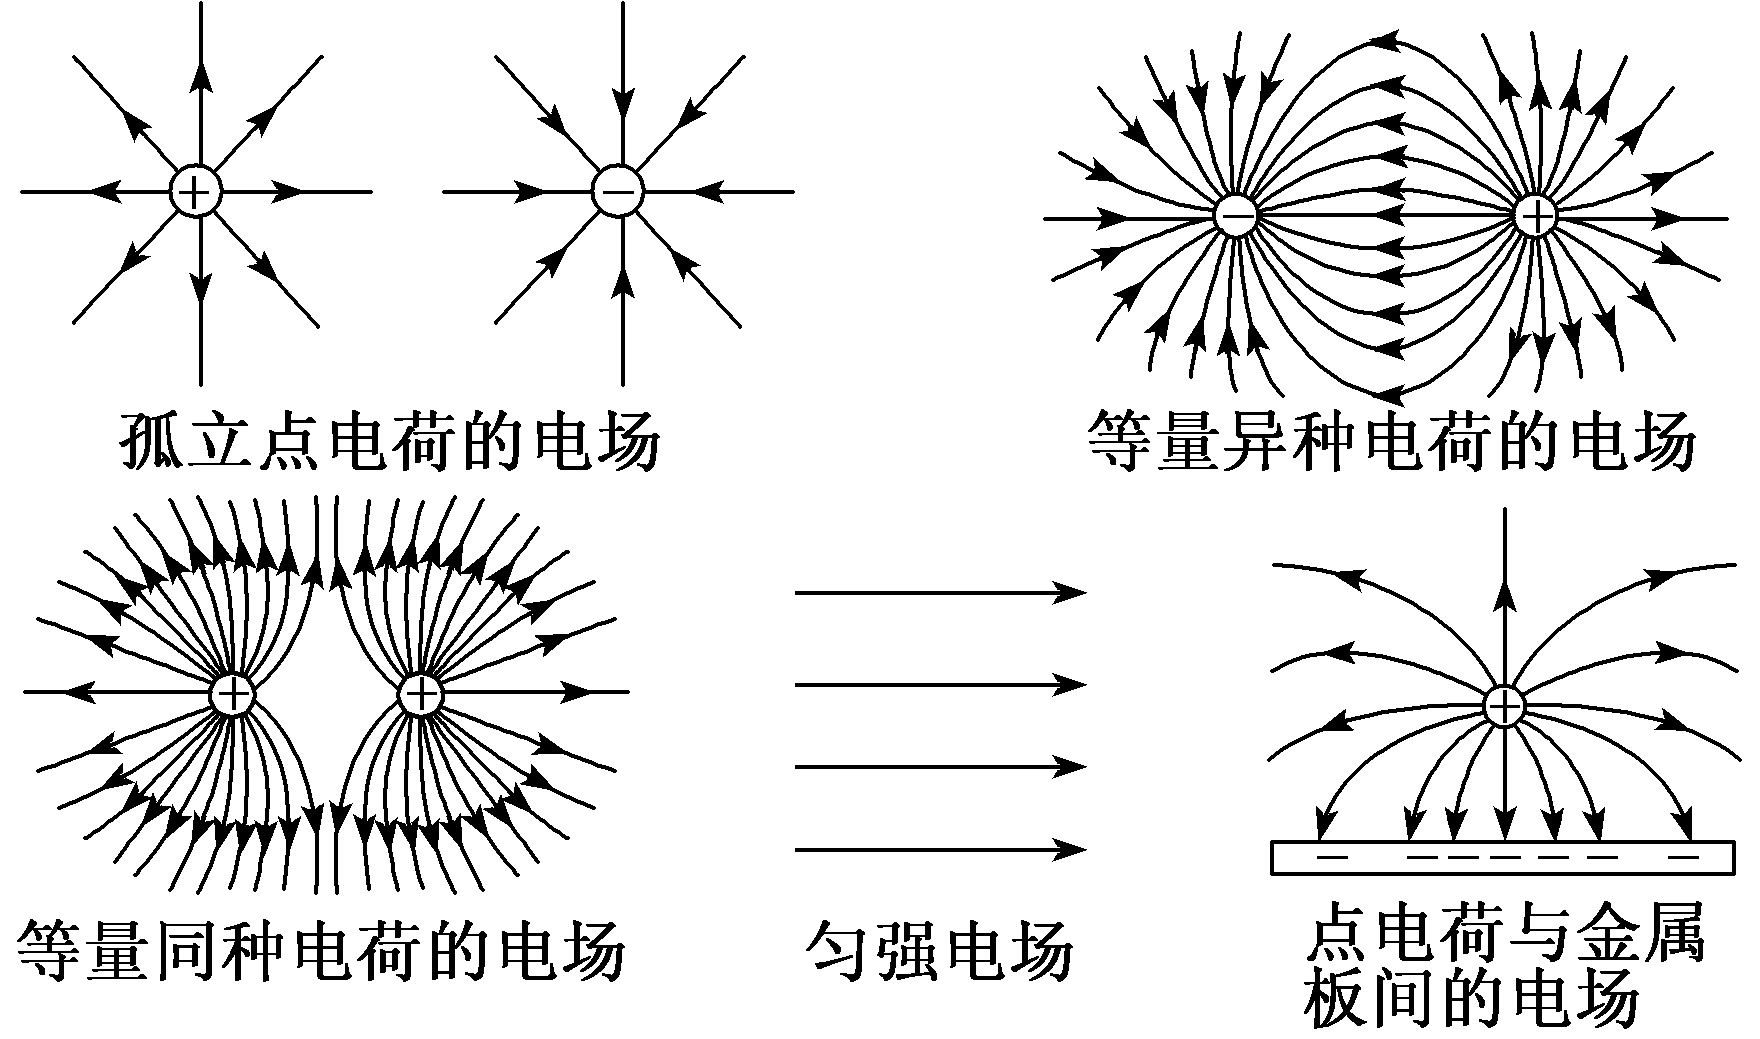
\includegraphics{./dianchang/dianchang1.png}
  \caption{六种常见的电场线}
  \label{fig:dianchangxian}
\end{figure}

在高中课本中给出了以上六种电场线的分布图,下面我们讨论一下这几个电场线的特点.

{\bf 孤立点电荷的电场}:此电场可以由公式计算.由真空中点库仑定律和电场强度的定义可得
\begin{gather}
  \left.
    \begin{gathered}
      F=k\frac{Qq}{r^2}\\
      E=\frac{F}{q}
    \end{gathered}
  \right\}
  \Longrightarrow
  E=k\frac{Q}{r^2}
\end{gather}

对于上式我们即可以按\CJKunderwave{标量式}来理解:即电荷量$Q$认为是其绝对值,而方向则单独记忆(正的点电荷激发的场强方向沿半径向外,负的点电荷激发的场强方向沿半径向里.),也可以按\CJKunderwave{矢量式}来记忆:沿半径方向向外为正,则$Q>0 , E>0$ 场强方向与正方向相同;如$Q<0,E<0$ 则场强方向与正方向相反.
\footnote{由于在电场这一部分的公式中出现的$q$ 有正电也有负电,为了不至于使用上的混乱,我建议同学位采用矢量式的方法记忆,这样今后所涉及的公式都需要$q$自身内部今有正负号,不需要再区分带不带正负号的问题.}
从公式上来看:\CJKunderwave{当r增大时,场强的大小会减小},从电场线上来看:\CJKunderwave{离点电荷越远,则电场线越稀疏,则场强的大小也越来越小},公式的描述和电场线的描述是一致的,但是电场线不能给出具体的数值,公式法可以给出具体数值,然而电场线较公式法的优点在于能够在整体上给出电场的分布情况.

{\bf 等量异种电荷的电场}:我们首先来看电场线中间连线上场强的分布情况,从电场线上来看由正电荷向负电荷电场线先变稀疏再变密集,所以场强是\CJKunderwave{先变小再变大,而且方向由正电荷指向负电荷}.这个情况,我们也可以根据电场的叠加从公式来看,如下

  设由正电荷指向负电荷方向为正,设两个电荷的距离为$2d$,设中间连线上的点距离正电荷为$r$,则中间连线上电场强度为 
  \begin{equation}
    E=k\frac{Q}{r^2}+k\frac{Q}{(2d-r)^2}
  \end{equation}

  从数学上不难判断,当半径 $r=d$ 时电场强度取得极大值.同时大家应当注意,此公式不能使 $r$ 从零开始变化,原因在于如果 $r\to 0$,则库仑公式失效,则此公式也失效,所以这时只能通过公式确定电场的变化情况和远离点电荷的电场强度大小.

  对于中垂线上电场强度的变化,从图中可以判断出来:从中间向两侧,电场强度逐渐减小.这里大家要注意,此处应当放眼整个立体空间来看,中垂线实际上是中垂面和纸面的交线,向两侧应当实指远离中点且在中垂面上.这也可以从公式上来分析.如下

  \begin{figure}[H]
    \centering
    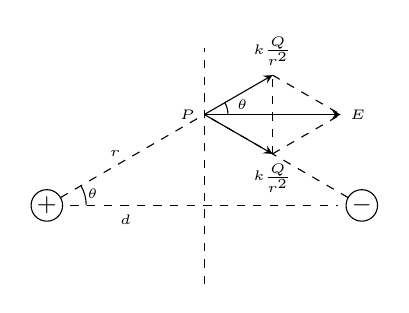
\begin{tikzpicture}
    \draw (-2,0) circle [radius=0.2] node {\small $+$};
    \draw (2,0) circle [radius=0.2] node {\small $-$};
    \draw[dashed] (-1.7,0)--(1.7,0);
    \draw[dashed] (0,-1)--(0,2);
    \draw[dashed] (-2,0)++(30:0.2)--++(30:2.1094);
    \draw[dashed] (2,0)++(150:0.2)--++(150:2.1094);
    \draw[->,>=stealth](0,1.1547)--++(30:1) node [anchor=south] {\tiny $k\frac{Q}{r^2}$};
    \draw[dashed](0,1.1547)++(30:1)--++(-30:1);
    \draw[->,>=stealth](0,1.1547)--++(-30:1) node [anchor=north] {\tiny $k\frac{Q}{r^2}$};
    \draw[dashed](0,1.1547)++(-30:1)--++(30:1);
    \draw[->,>=stealth](0,1.1547)--++(0:1.732) node [anchor=west] {\tiny $E$};
    \draw (-2,0)++(0:0.5) arc (0:30:0.5);
    \draw (-2,0)++(15:0.6) node {\tiny $\theta$};
    \draw (0,1.1547)++(0:0.3) arc (0:30:0.3);
    \draw (0,1.1547)++(15:0.5) node {\tiny $\theta$};
    \draw[dashed](0,1.1547)++(-30:1)--++(0,1);
    \draw (-1,0) node [anchor=north] {\tiny $d$};
    \draw (-2,0)++(30:1) node [anchor=south] {\tiny $r$};
    \draw (0,1.1547) node [anchor= east] {\tiny $P$};
    \end{tikzpicture}
    \caption{等量异种电荷中垂面上的场强}
    \label{fig:dengliangyizhongdianhe}
  \end{figure}

  对于中垂线上任意一点,由电场强度的叠加可得$P$点的场强,即
  \begin{gather}
    \left.
      \begin{gathered}
	E=2k\frac{Q}{r^2}\cos\theta\\
	r=\frac{d}{\cos\theta}
      \end{gathered}
    \right\}
    \Longrightarrow
    E=2k\frac{Q}{d^2}\cos^3\theta
  \end{gather}

  当场点由中间向两侧移动时,对应$\theta$ 将会变大,当无穷远时 $\theta=90^\circ$ ,当$0^\circ <\theta <90^\circ $ 时,$\theta$ 变大则 $\cos\theta$ 是减小的,所以中垂线上由中间向两侧电场强度逐渐减小直到为0.

  {\bf 等量同种电荷的电场}:从电场线的分布情况可以判断出来,在电荷的连线上电场强度先减小后增大,在中间位置为0,越过中点后场强改变方向,然后再增大.这一点也可以从公式来看,设向右为正,场点距左侧正电荷$r$ , 两电荷间距为 $2d$,则
  \begin{equation}
    E=k\frac{Q}{r^2}-k\frac{Q}{(2d-r)^2}
  \end{equation}
  当 $r<d$ 时 $E>0$ ,随 $r$ 增大则 $E$ 减小; 当 $r=d$ 时, $E=0$; 当 $r>d$ 时, $E<0$ , 随 $r$ 增大,则 $E$ 减小.这里也应当特别注意,$r\to 0$ 时,库仑定律失效,所以这里讨论的场强也不能是紧挨场源电荷的.

  对于中垂线上电场强度的变化,从图中可以判断出来:由于中间场强为$0$ , 在无穷远处场强也为 $0$ ,但是中垂线上除这两处外不是 $0$ ,因此场强的变化应当是先增大再减小.我们可以具体算出最大场强的位置,高一的同学暂时没有学习求导函数法求极值,计算暂时可以略过,但是待数学知识完备后,一定要回来具体计算一下此最大场强.具体计算如下

  \begin{figure}[H]
    \centering
    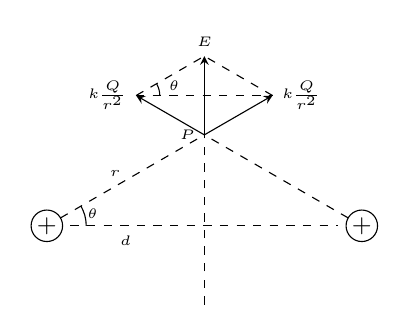
\begin{tikzpicture}
    \draw (-2,0) circle [radius=0.2] node {\small $+$};
    \draw (2,0) circle [radius=0.2] node {\small $+$};
    \draw[dashed] (-1.7,0)--(1.7,0);
    \draw[dashed] (0,-1)--(0,2);
    \draw[dashed] (-2,0)++(30:0.2)--++(30:2.1094);
    \draw[dashed] (2,0)++(150:0.2)--++(150:2.1094);
    \draw[->,>=stealth](0,1.1547)--++(30:1) node [anchor=west] {\tiny $k\frac{Q}{r^2}$};
    \draw[dashed](0,1.1547)++(30:1)--++(150:1);
    \draw[->,>=stealth](0,1.1547)--++(150:1) node [anchor=east] {\tiny $k\frac{Q}{r^2}$};
    \draw[dashed](0,1.1547)++(150:1)--++(30:1);
    \draw[->,>=stealth](0,1.1547)--++(90:1) node [anchor=south] {\tiny $E$};
    \draw (-2,0)++(0:0.5) arc (0:30:0.5);
    \draw (-2,0)++(15:0.6) node {\tiny $\theta$};
    \draw (0,1.1547)++(150:1)++(0:0.3) arc (0:30:0.3);
    \draw (0,1.1547)++(150:1)++(15:0.5) node {\tiny $\theta$};
    \draw[dashed](0,1.1547)++(150:1)--++(1.732,0);
    \draw (-1,0) node [anchor=north] {\tiny $d$};
    \draw (-2,0)++(30:1) node [anchor=south] {\tiny $r$};
    \draw (0,1.1547) node [anchor= east] {\tiny $P$};
    \end{tikzpicture}
    \caption{等量同种电荷中垂面上的场强}
    \label{fig:dengliangtongzhongdianhe}
  \end{figure}
  对于中垂线上任意一点,由电场强度的叠加可得$P$点的场强,即
  \begin{gather}
    \left.
      \begin{gathered}
	E=2k\frac{Q}{r^2}\sin\theta\\
	r=\frac{d}{\cos\theta}
      \end{gathered}
    \right\}
    \Longrightarrow
    E=2k\frac{Q}{d^2}\cos^2\theta\sin\theta\notag
    \intertext{上式可以写成关于$\sin\theta$ 的函数,即}
    E=2k\frac{Q}{d^2}(1-\sin^2\theta)\sin\theta\notag
    \intertext{上式对$\sin\theta$ 微分,令其微分为$0$ ,则}
    \frac{d E}{d\sin\theta}=2k\frac{Q}{d^2}(1-3\sin^2\theta)=0\notag
    \intertext{解得最大电场强度出现的位置为}
    \sin\theta=\frac{\sqrt{3}}{3}\notag
  \end{gather}
    同学们注意,上式所求$\theta$ 可不是一个特殊值,它是\CJKunderdot{正弦值}为$\frac{\sqrt{3}}{3}$ 而\CJKunderdot{不是正切值}!!

  {\bf 匀强电场}:匀强电场的电场线是等间距的平行线,等间距表明电场强度大小不变,平行表明方向在任何位置都一样.如果需要计算场强,也得在平行板电容器中才行,有的题目也会借助受力平衡的问题拐个弯用定义等来求匀强电场的大小,一般而言它是给定的,然后让同学们去求解力和运动的问题.对于最后一个,真空中的点电荷和无限大平行金属板间的电场,可以借助于镜像法来求解电势再微分来得到电场强度,但是这已经超出了高中对同学们的要求,所以此处不再具体计算.有高考题,曾经考过此类问题,但是结合电场的叠加和对称性可以方便的解决,当遇到具体问题时再做分析.

  \section{电势能和电势}

  电场是我们新认识的一种物质,当电荷放入电场中时会受到力的作用,所以当将电荷从一个位置移动到另一个位置时电场力有可能做功,但是根据能量守恒定律,这就涉及到能量的转化.但是由于电荷及电场有它自己特定的特点,同时电场大多数的情况下又不是恒力,这就不能像重力那样确定重力势能.实践表明,电荷放入电场中也有势能,我们称之为电势能.但是没有经过严格的数学论证前我们还不能肯定这个结论.有的教材上类比``重力场''来说明电场和电势能,但是我要问一句,我们哪一本书上在讲解重力时提到过重力场?同学们根本没有听过重力场\footnote{至少在高中一年级是这样的,这也是我从电荷和电场本质属性来讨论问题的原因.},所以我不想那样讲解,根据前面几节学过的内容我们可以顺理成章的给出电势能.

  一种势能的存在必然表明此势能只能是位置的函数,那就是做功与路径无关,在物理学上我们称做功与路径无关的力为\CJKunderwave{保守力}.

  \subsection{静电力是保守力}

  静电力做功也与路径无关,所以它是保守力.由于电场的复杂性,我们对于任意一个电场来讲,先来考虑一个很小很小的区域,则在这一个小区域内电场几乎没有变化,可以视为匀强电场.如图\ref{fig:yuqiangdianchanglujingwufuang} 所示

  \begin{figure}[H]
    \centering
    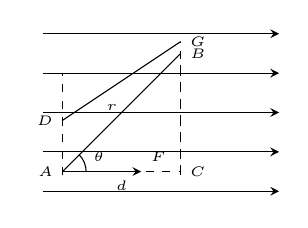
\begin{tikzpicture}
      \foreach \y in {0,0.5,1,1.5,2}
      \draw [->,>=stealth] (0,\y)--(3,\y);
      \draw (0.25,0.25) node [anchor=east] {\tiny $A$}--(1.75,1.75) node [anchor=west] {\tiny $B$};
      \draw[dashed] (0.25,0.25)--(1.75,0.25) node [anchor=west]{\tiny $C$}--(1.75,1.75);
      \draw (0.55,0.25) arc (0:45:0.3);
      \draw (0.25,0.25)++(22.5:0.5) node {\tiny $\theta$};
      \draw (1,0.25) node [anchor=north] {\tiny $d$};
      \draw (45:1.5) node [anchor=east]{\tiny $r$};
      \draw[->,>=stealth] (0.25,0.25)--++(0:1) node [anchor=south west]{\tiny $F$};
      \draw (0.25,0.9)node [anchor=east] {\tiny $D$} --(1.75,1.9) node [anchor=west]{\tiny $G$};
      \draw [dashed] (0.25,0.2)--(0.25,1.5);
      \draw [dashed] (1.75,0.2)--(1.75,1.9);
    \end{tikzpicture}
    \caption{匀强电场做功与路径无关}
    \label{fig:yuqiangdianchanglujingwufuang}
  \end{figure}

  我们将电荷 $q$ 沿路径 $AB$ 由 $A$ 移动到 $B$ ,计算静电力做功,则
  \begin{equation}
    W_{AB}=qEr\cos\theta
    \label{eq:jdlwork0}
  \end{equation}
  然后,我们再沿路径 $A\to C\to B$ 将电荷 $q$ 由 $A$ 移动到 $B$,计算静电力做功,则
  \begin{equation}
    W_{AB}'=W_{AC}+W_{CB}=qEd+0
    \label{eq:jdlwork1}
  \end{equation}
  对比式 \eqref{eq:jdlwork0} 和 \eqref{eq:jdlwork1} 由几何关系可得 $r\cos\theta  =d$ 所以有
  \begin{equation}
    W_{AB}=W_{AB}'
    \label{eq:jdlwork2}
  \end{equation}
  上式表明:\CJKunderwave{匀强电场中,静电力做功与路径无关.}同理也可以确定将电荷沿$DG$ 路径由 $D$ 移动到 $G$ ,静电力做功也等于$W_{AB}'$ .所以有
  \begin{equation}
    W_{AB}=W_{DG}
    \label{eq:jdlwork3}
  \end{equation}
  式 \eqref{eq:jdlwork3} 可得:在匀强电场中,只要两点沿\CJKunderwave{沿电场线方向的距离相等},则电场对电荷做功相等.

  对于一般的情况,如图 \ref{fig:yibanjdlwork},我们将路径沿电场线方向做出一定划分,每一个小区域可以视为匀强电场.路径$A\to D\to B$ 和路径 $A\to C\to B$ 离的非常近,所以按图中每隔一小段画一小条虚线与电场线(电场线未画出)垂直,由匀强电场的第二条规律:\CJKunderwave{在匀强电场中,只要两点沿沿电场线方向的距离相等,则电场对电荷做功相等.}可得第一小段上静电力做功相等,所以沿路径$A\to C\to B$ 和路径 $A\to D\to B$计算静电力做功是相同的,如果两条路径相隔比较远,则可以通过若干相邻路径逐步得到,所以可以断言:任何静电场中,静电力做功与路径无关,只取决于始末位置.


  \begin{figure}[H]
    \centering
    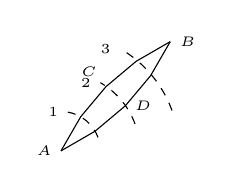
\begin{tikzpicture}
      \draw (0,0) node [anchor=east] {\tiny $A$}--++(60:0.5)--++(50:0.5) node [anchor= south east] {\tiny $C$}--++(40:0.5)--++(30:0.5) node [anchor=west] {\tiny $B$};
      \draw (0,0)--++(30:0.5)--++(40:0.5) node [anchor=west] {\tiny $D$}--++(50:0.5)--++(60:0.5);
      \draw[dashed] (20:0.5) arc (20:80:0.5) node [anchor=east] {\tiny 1};
      \draw[dashed] (20:1) arc (20:60:1) node [anchor=east] {\tiny 2};
      \draw[dashed] (20:1.5) arc (20:60:1.5) node [anchor=east] {\tiny 3};
    \end{tikzpicture}
    \caption{一般电场的情况}
    \label{fig:yibanjdlwork}
  \end{figure}

  \subsection{电势能}
  由于静电力是保守力,所以由静电力做功与路径无关可以判断静电力做功只与始末位置有关,这是上一节的结论.由于$W_{AB}$ 只与始末位置有关,所以它可以表达为两个函数的差的形式,这个函数我们就称为电势能.即
  \begin{equation}
    W_{AB}=E_{pA}-E_{pB}
    \label{eq:dianshineng}
  \end{equation}

  式\eqref{eq:dianshineng}将\CJKunderwave{静电力做功表达为电势能的减少量},但是具体的电势能的数值还没有确定下来,这就需要人为的选定.由式\eqref{eq:dianshineng} 可以得出,如果我们选定 $E_{pB}=0 J$ ,则
  \begin{equation}
    E_{pA}=W_{AB}
    \label{eq:dianshineng1}
  \end{equation}
  式\eqref{eq:dianshineng1}可得一条重要的结论:\CJKunderwave{某点的电势能等于将电荷从该点移动到零势能点静电力做的功.}

  \subsection{电势}

  不同的电荷放在同一个电场中的相同位置,它们的受力是不一样的,所以移动时静电力做功也不一样,则电势能也不相同.所以可以判断电势能与电荷量有关,不能表示电场自身的性质,同时由于电场的多样性,也不可能找出一个和重力势能一样的简单的表达式.但是电荷它有自己的特点,即:\CJKunderwave{所有的电荷量都是元电荷的整数倍}. 由于这个特点,我们可将电荷 $q$ 从 $A$ 点移动到 $B$ 点计算电场力做功时,可以一次性的移动过去,也可以分成若干次,每次只移动一个元电荷$e$ ,于是可以得出结论:\CJKunderwave{从 $A$ 到 $B$ 静电力做功与移动的次数成正比,同时由电势能的定义可以断定电势能也与这个移动次数成正比,}即设移动次数为 $N$ ,则 $N=\frac{q}{e}$,所以可以得出 $E_p$ 和电荷量 $q$ 成正比,定义此比例系数为\CJKunderwave{电势},使用符号$\varphi$ \footnote{$\varphi$ 是希腊字母,同学们要准确的书写不要与英文字母弄混,这点特别引起注意.}表示,则其定义为
  \begin{equation}
    \varphi=\frac{E_p}{q}
    \label{eq:dianshi}
  \end{equation}
  式\eqref{eq:dianshi} 表明,电势是一个标量,符合比值定义法,其不依赖于电场中所放置的电荷,所以电势可以表征\CJKunderwave{电场自身的属性}.对于比值定义法,在这里有必要解释一下,因为平时的教学中很多学生总是在这里出问题.举一例来说明,比如远古时代并没有钱,但是随着社会发展出现了货币,也就是钱!但是由于钱的特殊作用,以及重要性,人们需要专门的找一个包来存放它,慢慢的大家就给放钱的这个包起了一个名字---钱包.这里你看,钱包是用钱来定义的,但是它和钱绝对不是一个东西,而且一个钱包的存钱能力(容积大小)和它里面有没有钱也是没有关系的!所以电势虽然是由电荷放入电场中时所具有的电势能和电荷量的比值来定义的,但它和放入其中的电荷是没有关系的,所以它代表了电场自身能的性质! 如果我们再深入一些找一下决定电势的因素,则电场是由场源电荷激发的,所以它取决于场源电荷,同时电场一定的情况下,电势也不是确定的,因为还需要人为的指定零电势能的位置(也可以说是零电势位置).

  电势是一个标量,它的单位是:伏特,符号为 V .\footnote{大家注意,这里的伏特就是初中时大家学习的电压的单位,但是电势又不是电压,这需要在后面的课程中解释.}

  \section{电势差}

  前面我们介绍了电势能的概念和电势的概念,但是在计算一般情况下静电力做功时,并不总是很实用,原因在于如果每次计算都先选择零势能面,会带来不必要的计算.考虑到这个因素,我们引入一个新的物理量---电势差.定义如下
  \begin{equation}
    U_{AB}=\varphi_A-\varphi_B
    \label{eq:dianshicha}
  \end{equation}

  注意定义\eqref{eq:dianshicha} 中下脚标的顺序,$AB$不能颠倒.由这定义可以得到下面的二个性质
  \begin{gather}
    U_{AB}=-U_{BA}\\
    U_{AC}=U_{AB}+U_{BC}
  \end{gather}
  上述性质是显然的,由电势差的定义不难证明,这里留给同学们自己完成证明,不再辍述.

  我们再来讨论一下静电力做功与电势差的关系.如下
  \begin{gather}
    \left.
    \begin{gathered}
    W_{AB}=E_{pA}-E_{pB}\\
    E_p=q\varphi\\
    U_{AB}=\varphi_A-\varphi_B
    \end{gathered}
  \right\}
  \Longrightarrow
  U_{AB}=\frac{W_{AB}}{q}
  \label{eq:WandU}
  \end{gather}

  关系式 \eqref{eq:WandU} 可以用来知道电势差的情况下直接计算功,也可以知道功的情况下直接计算电势差,由于它不涉及零势能面的选择,所以使用起来比较方便.

  \section{电场强度和电势差的关系}

  现在讨论一个特殊,在匀强电场中电场力是恒力,所以它做的功可以直接算出,因而可以得到一个非常好用的关系式.在讨论匀强电场中静电力做功的时候我们得到从$A$ 到 $B$ 静电力做功为$W_{AB}$,$d$ 表示沿电场线方向 $AB$ 的距离.将其应用于电势差的计算式中,即
  \begin{gather}
    \left.
      \begin{gathered}
	W_{AB}=qEd \\
	U_{AB}=\frac{W_{AB}}{q}
      \end{gathered}
    \right\}
    \Longrightarrow
    U_{AB}=Ed
    \label{eq:EanU}
  \end{gather}
  为了更好的理解方向和它们之间的关系,我们沿电场线方向建立一维直线坐标系,则如图\ref{fig:PhiAndE}所示,由电势差的定义,我们可以把场强与电势差的关系写为
  \begin{equation}
    E=-\frac{\varphi_B-\varphi_A}{x_B-x_A}=-\frac{\Delta\varphi}{\Delta x}
    \label{eq:EandU1}
  \end{equation}
\begin{figure}[H]
  \centering
  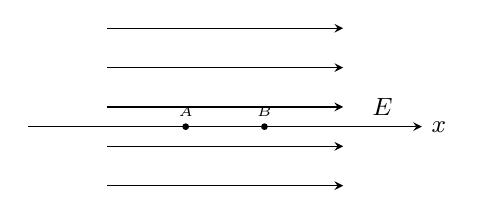
\begin{tikzpicture}
    \foreach \y in {0,0.5,1,1.5,2}
    \draw [->,>=stealth] (0,\y)--(3,\y);
    \draw (3.5,1) node {\small $E$};
    \draw [->,>=stealth] (-1,0.75)--(4,0.75) node [anchor=west] {\small $x$};
    \filldraw (1,0.75) node [anchor=south] {\tiny $A$} circle [radius=1pt];
    \filldraw (2,0.75) node [anchor=south] {\tiny $B$}circle [radius=1pt];
  \end{tikzpicture}
  \caption{电场强度与电势差的关系}
  \label{fig:PhiAndE}
\end{figure}

\section{电容器的电容}

我们学习了起电的方式,找到了能够得到净电荷的方法.但是由于开始并不清楚电荷及电场的有关特点,所以尚没有解决电荷存储的问题.这一节所解决的就是电荷存储的问题.\CJKunderwave{能够存储电荷的\CJKunderdot{设备}叫做\CJKunderdot{电容器}}.电容器存储电荷的基本原理是:异种电荷相互吸引.如果将两个导体之间充以绝缘介质,则当两个导体上分别使其带上异种电荷时,由于异种电荷间的相互吸引,同时它们之间又是绝缘的,电荷还不能中和,所以最后只能分别在两个导体上了,而且最终也必然会保持电荷在宏观上的静止状态.
\begin{figure}[H]
  \centering
  \begin{tikzpicture}
    \draw (-0.2,0) rectangle (3.2,0.2); 
    \draw (-0.2,2) rectangle (3.2,2.2); 
    \foreach \x in {0,0.5,1,1.5,2,2.5,3}
    \draw (\x, 0.1) node {\tiny $-$};
    \foreach \x in {0,0.5,1,1.5,2,2.5,3}
    \draw (\x, 2.1) node {\tiny $+$};
    \foreach \x in {0,0.5,1,1.5,2,2.5,3}
    \draw[->,>=stealth] (\x,1.95) -- (\x, 0.25);
    \draw (1.5,1.1) node {\small 绝缘介质};
  \end{tikzpicture}
  \caption{平行板电容器}
  \label{fig:pingyxingban}
\end{figure}

如图 \ref{fig:pingyxingban} 所示,是最简单的一种电容器,它有两个无限大金属板中间填充绝缘介质构成,所以叫做平行板电容器.如果我们将两个极板同时和电源的正负两极连接,则两个极板上就会充上等量异种电荷,我们把这个过程叫做电容器的充电.图中正是表示的充电后的状态.如果我们把一个充电的电容器的两极用一根导线连接,则正负电荷就会通过导线中和,从而二个极板不再带电,我们称这个过程为电容器的放电.由这个特点我们可以肯定的是电容器的容量是指\CJKunderwave{一个极板上的电荷量的绝对值.}

就像水杯一样,水杯是盛水的容器,不同的水杯有不同的容积,也就是有不同的水的容纳能力.电容器也是一样,不同的电容器对电荷的容纳能力也是不一样的,所以就产生了如何衡量电容器电荷容纳能力的问题.当有电场时,即便是绝缘介质,它不导电,但是由于原子是电中性,电场会使其中的正负电荷向相反的方向偏离,但是由于原子内部正负电荷的吸引,最终会和外部的电场力平衡掉.但是确改变了原子的形状!原则上讲,只要是外电场足够强大,就能使绝缘介质的原子中的正负电荷分开,我们称之为电离.因此,只有在绝缘介质不发生电离时,电容器才是完好的,其两个极板上的电荷才不会中和,而得以存储.所以这里就存在一个电容器中所能允许的最大场强问题,也就是电场线的密度不能超过一个值,然而电荷又都是元电荷的整数倍,所以可以认为每一个元电荷对就一条电场线,由于电场线的条数在正对面积一定的情况下有一个极大值,则一个极板上的电荷量也必然有一个极大值,也就是说电容器极板上的电荷量也是有限制的.同时根据 
$U=Ed$ 可得,在两板间距离 $d$ 一定的情况下,电压也是存在一个上限的,我们称之为额定电压.

当一个电容器制成后,如果增加极板上的电荷量,则极板间的电压也跟着增加,同时场强也增加,但是如果两个电容器充以相同的电介质,当增加相同的电量时,增加电压少的那一个意味着电场强度增加的也少,意味着更不容易导致介质电离,也就是电荷容纳本领越大.所以可以使用电荷量与板间电压的比值来表示电容器容纳电荷的本领,定义为电容,即
\begin{equation}
  C=\frac{Q}{U}
  \label{eq:dianrong}
\end{equation}
由定义可知,电容是一个标量.电容的国际单位是:法拉,符号为:$F$. 法拉是一个极大的单位,日常中常见电容器的电容一般都达不到这么大,所认还有两个更小的单位皮法$pF$ 和微法 $\mu F$,它们之间的进位为
\begin{equation}
  1F=10^6 pF = 10^{12} \mu F
  \label{eq:falajinwei}
\end{equation}

综上讨论,我们可以得出一些结论,在一个极板上电荷量一定的情况下,如果正对面积越大,则电场线密度越低,则电容器容纳电荷的本领越大.同时在相同介质的前提下,两个极板间距离越大则两个电荷间的库仑力越小,则保持电荷稳定保存的能力就越低,所以板间距离越大,则电容器容纳电荷的本领就越小.同时电容器不易电离的能力,也即是绝缘能力越大则该电容器的容纳电荷的本领越大.以 $S$ 表示极板正对面积, 以 $d$ 表示板间距离, 以 $\varepsilon_r$ 表示相对介电常数\footnote{$\varepsilon$ 为介质的介电常数, $\varepsilon_0$ 为真空中的介电常数,相对介电常数定义为 $\varepsilon_r=\frac{\varepsilon}{\varepsilon_0}$ ,它们是衡量物质绝缘性能的物理量,其值越大,则绝缘性能越好.},所以我们可以推断出来平行板电容器的电容和正对面各成正比,和板间距离成反比,和相对介电常数成正比,即 $C\propto \frac{\varepsilon_r S}{d}$ ,严格计算的结果为
\begin{equation}
  C=\frac{\varepsilon_r S}{4\pi k d}
  \label{eq:dianrongpingban}
\end{equation}
上式中$k$ 为静电力常量,其值为$k=9.0\times 10^9 N\cdot m^2/C^2$.
\section{带电粒子在电场中的运动}

\subsection{带电粒子的加速}

当带电粒子在电场中运动时,高中最常处理的也是最基本的就是带电粒子的加速问题.如图
\ref{fig:ddlzjiasu}所示,两板间电压为$U_1$, 平行板间距离为$d_1$,粒子的带电量为$q$,质量为$m$.

\begin{figure}[H]
  \centering
  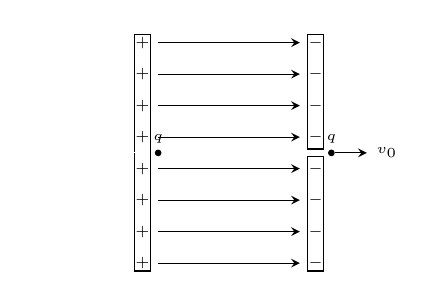
\begin{tikzpicture}
    \draw (-0.2,-1.5) rectangle (0,1.5); 
    \draw (2,-1.5) rectangle (2.2,-0.05); 
    \draw (2,0.05) rectangle (2.2,1.5); 
    \foreach \y in {-1.4,-1.0,-0.6,-0.2,0.2,0.6,1.0,1.4}
    \draw (-0.1,\y) node {\tiny $+$};
    \foreach \y in {-1.4,-1.0,-0.6,-0.2,0.2,0.6,1.0,1.4}
    \draw (2.1,\y) node {\tiny $-$};
    \foreach \y in {-1.4,-1.0,-0.6,-0.2,0.2,0.6,1.0,1.4}
    \draw[->,>=stealth] (0.1,\y)--(1.9,\y);
    \filldraw (0.1,0) circle [radius=1pt] node [anchor=south]{\tiny $q$};
    \filldraw (2.3,0) circle [radius=1pt] node [anchor=south]{\tiny $q$};
    \draw[->,>=stealth] (2.35,0)--(2.75,0) node [anchor=west]{\tiny $v_0$};
    \draw[color=white](-1.55,0)--(0,0);
  \end{tikzpicture}
  \caption{带电粒子在电场中加速}
  \label{fig:ddlzjiasu}
\end{figure}

下面我们来求带电粒子离开加速电场时的速度$v_0$,由动能定理得
\begin{gather}
  qU=\frac{1}{2}mv_0^2
  \intertext{解得}
  v_0=\sqrt{\frac{2qU_1}{m}}
  \intertext{如果要求粒子的加速时间,则需要考虑运动学公式,由平均速度公式得}
  d_1=\frac{v_0}{2}t
  \intertext{解得}
  t=\frac{2d_1}{v_0}=d_1\cdot\sqrt{\frac{2m}{qU_1}}
  \intertext{此题也可以由匀变速直线运动来求解.由牛顿第二定律得}
  q\frac{U_1}{d_1}=ma_1
  \intertext{解得}
  a_1=\frac{qU}{md_1}
  \intertext{由匀变速直线运动位移与时间的关系可得}
  d_1=\frac{1}{2}a_1t^2
  \intertext{解得}
  t=\sqrt{\frac{2d_1}{a_1}}=d_1\cdot\sqrt{\frac{2m}{qU_1}}
\end{gather}

\subsection{带电粒子在电场中的偏转}

这一节讨论带电粒子在电场中的偏转问题,由于高中的要求,此处仅讨论类平抛运动.如图\ref{fig:ddlzpz}所示,两板间电压为$U_2$,板长为$L$.

\begin{figure}[H]
  \centering
  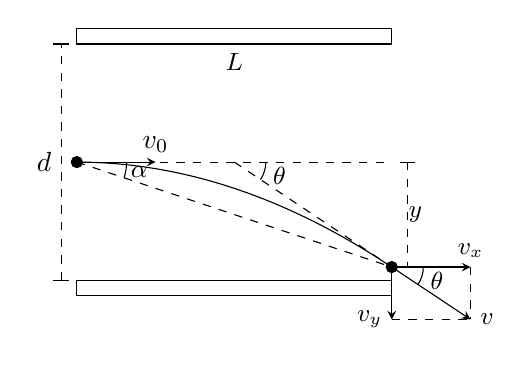
\begin{tikzpicture}
    \draw (-2,-1.7) rectangle (2,-1.5); 
    \draw (-2,1.7) rectangle (2,1.5); 
    \draw[dashed] (-2,0)--(2,0);
    \draw[domain=-2:2] plot (\x,-\x*\x/12-\x/3-1/3);
    \draw[->,>=stealth] (-2,0)--(-1,0) node [anchor=south]{$v_0$};
    \filldraw (-2,0) circle [radius=2pt];
    \draw[dashed](0,0)--(2,-1.333);
    \filldraw (2,-1.333) circle [radius=2pt];
    \draw[->,>=stealth] (2,-1.333)--++(1,-0.666) node [anchor=west]{\small $v$};
    \draw[->,>=stealth] (2,-1.333)--++(1,0) node [anchor=south]{\small $v_x$};
    \draw[->,>=stealth] (2,-1.333)--++(0,-0.666) node [anchor=east]{\small $v_y$};
    \draw[dashed](2,-1.333)++(1,0)--++(0,-0.666);
    \draw[dashed](2,-1.333)++(0,-0.666)--++(1,0);
    \draw[dashed](-2,0)--(2,-1.333);
    \draw (-2,0)++(0.6,-0.1998) arc (-18.433:0:0.6);
    \draw (-2,0)++(-9.22:0.8) node {\small $\alpha$};
    \draw(2,-1.333)++(-33.6874:0.4) arc (-33.6874:0:0.4);
    \draw(0,0)++(-33.6874:0.4) arc (-33.6874:0:0.4);
    \draw(2,-1.333)++(-16.8437:0.6) node {\small $\theta$}; 
    \draw(0,0)++(-16.8437:0.6) node {\small $\theta$}; 
    \draw (0,1.5) node [anchor=north]{\small $L$};
    \draw (-2.3,1.5)--(-2.1,1.5);
    \draw (-2.3,-1.5)--(-2.1,-1.5);
    \draw[dashed] (-2.2,-1.5)--(-2.2,1.5);
    \draw (-2.2,0) node [anchor=east]{$d$};
    \draw (2.1,0)--(2.3,0);
    \draw (2.1,-1.333)--(2.3,-1.333);
    \draw[dashed](2.2,0)--(2.2,-1.333);
    \draw (2.3,-0.666) node {\small $y$};
  \end{tikzpicture}
  \caption{带电粒子在电场中偏转}
  \label{fig:ddlzpz}
\end{figure}

\subsubsection{偏转加速度}

由牛顿第二定律可得
\begin{gather}
  q\frac{U_2}{d}=ma_2
  \intertext{解得}
  a_2=\frac{qU_2}{md}
  \label{eq:ddpya}
\end{gather}
上述结果同学位要记住,它很有规律,而且一旦记住能够实现快速写出偏转问题中的偏移量和偏转角等.

\subsubsection{偏移量}

图\ref{fig:ddlzpz} 中所示,带电粒子射出电场时相对于入射方向的纵向位移就叫做偏移量.由运动的独立性可得运动的时间为
\begin{gather}
  t=\frac{L}{v_0}
  \label{eq:ddpyl0}
  \intertext{所以偏移量为}
  y=\frac{1}{2}a_2t^2
  \label{eq:ddpyl1}
  \intertext{将式\eqref{eq:ddpya}和\eqref{eq:ddpyl0}代入\eqref{eq:ddpyl1}后得}
  y=\frac{1}{2}\cdot\frac{qU_2}{md}\cdot\frac{L^2}{v_0^2}
  \label{eq:ddpyl2}
\end{gather}

\subsubsection{位移偏转角}

由图\ref{fig:ddlzpz} 可得位移的偏转角为
\begin{gather}
  \tan\alpha=\frac{y}{L}=
  \frac{1}{2}\cdot\frac{qU_2}{md}\cdot\frac{L}{v_0^2}
  \label{eq:ddpyl3}
\end{gather}

\subsubsection{出射速度}

由运动学公式可得
\begin{gather}
  v_y=a_2t=\frac{qU_2}{md}\cdot\frac{L}{v_0}
  \intertext{由运动的合成可得}
  v=\sqrt{v_0^2+v_y^2}
  \intertext{这个出射速度也可以由动能定理求得,即}
  q\frac{U_2}{d}y=\frac{1}{2}mv^2-\frac{1}{2}mv_0^2
\end{gather}
 但是请同学们注意,在已经求得运动的时间和加速度的前提下,此处的动能定理走了弯路,原因在于偏移量本来就是由运动学公式求出来的,再代入动能定理运算会增加计算量.所以直接由运动的合成来求更方便.

\subsubsection{出射速度偏转角}

由图\ref{fig:ddlzpz} 及运动的合成和分解可得
\begin{gather}
  \tan\theta=\frac{v_y}{v_0}=\frac{qU_2}{md}\cdot\frac{L}{v_0^2}  
  \label{eq:ddpyl4}
\end{gather}

\subsubsection{位移偏转角和速度偏转角的关系}

对比式\eqref{eq:ddpyl4}和式\eqref{eq:ddpyl3}可得二个偏转角的正切值满足二倍关系.

\begin{gather}
  \tan\theta=2\tan\alpha
\end{gather}
注意:此处的二倍关系在平抛运动的计算中出现过.这是一个数学结论,只要轨迹是二次曲线,则它的切线与$x$轴的交点就是二次曲线顶点到所求切线的这一点的中点.可以证明如下:

\begin{figure}[H]
  \centering
  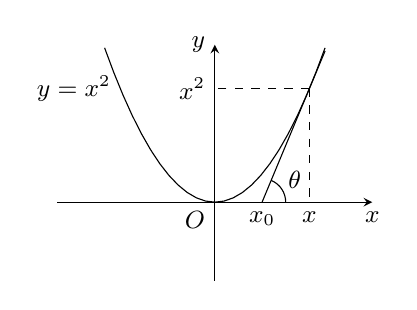
\begin{tikzpicture}
    \draw[->,>=stealth] (-2,0)--(2,0) node [anchor=north]{\small $x$}; 
    \draw[->,>=stealth] (0,-1)--(0,2) node [anchor=east]{\small $y$}; 
    \draw[domain=-1.4:1.4] plot (\x,\x*\x);
    \draw[dashed](1.2,1.44)--(1.2,0);
    \draw[dashed](1.2,1.44)--(0,1.44);
    \draw (0.6,0)--(1.2,1.44)--++(0.2,0.48);
    \draw (0.6,0)++(0.3,0) arc (0:67.38:0.3);
    \draw (0.6,0)++(33.69:0.5) node {\small $\theta$};
    \draw (1.2,0) node [anchor=north]{\small $x$};
    \draw (0.6,0) node [anchor=north]{\small $x_0$};
    \draw (0,1.44) node [anchor=east]{\small $x^2$};
    \draw (0,0) node [anchor=north east]{\small $O$};
    \draw (-1.2,1.44) node [anchor=east]{\small $y=x^2$};
  \end{tikzpicture}
  \caption{二倍关系论证}
  \label{fig:twobei}
\end{figure}
数学上容易求得切线的斜率,即对函数求导数
\begin{gather}
  \tan\theta=y'=2x
  \intertext{反向延长切线,交$x$轴于$x_0$,则由几何关系可得}
  \tan\theta=\frac{x^2}{x-x_0}
  \intertext{二者联立求得}
  x_0=\frac{1}{2}x
\end{gather}
所以$x_0$就是顶点$O$和坐标点$x$的中点.
\subsection{带电粒子加速和偏转的联合作用}
当一个粒子依次通过加速电场和偏转电场时,会有一些特殊的规律.这一节讨论这些特点.如图\ref{fig:ddlzjspz}所示,设加速电压为$U_1$,偏转电压为$U_2$.

\begin{figure}[H]
  \centering
  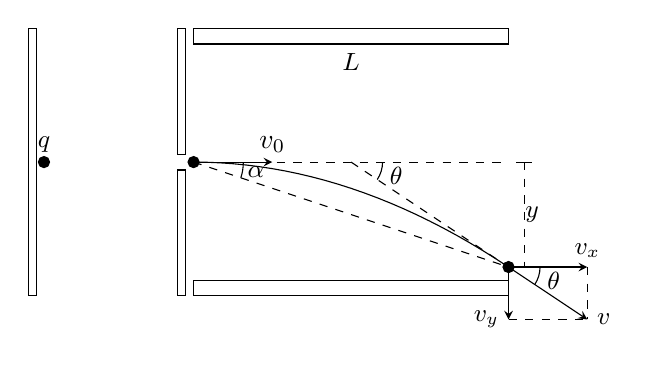
\begin{tikzpicture}
    \draw (-2,-1.7) rectangle (2,-1.5); 
    \draw (-2,1.7) rectangle (2,1.5); 
    \draw[dashed] (-2,0)--(2,0);
    \draw[domain=-2:2] plot (\x,-\x*\x/12-\x/3-1/3);
    \draw[->,>=stealth] (-2,0)--(-1,0) node [anchor=south]{$v_0$};
    \filldraw (-2,0) circle [radius=2pt];
    \draw[dashed](0,0)--(2,-1.333);
    \filldraw (2,-1.333) circle [radius=2pt];
    \draw[->,>=stealth] (2,-1.333)--++(1,-0.666) node [anchor=west]{\small $v$};
    \draw[->,>=stealth] (2,-1.333)--++(1,0) node [anchor=south]{\small $v_x$};
    \draw[->,>=stealth] (2,-1.333)--++(0,-0.666) node [anchor=east]{\small $v_y$};
    \draw[dashed](2,-1.333)++(1,0)--++(0,-0.666);
    \draw[dashed](2,-1.333)++(0,-0.666)--++(1,0);
    \draw[dashed](-2,0)--(2,-1.333);
    \draw (-2,0)++(0.6,-0.1998) arc (-18.433:0:0.6);
    \draw (-2,0)++(-9.22:0.8) node {\small $\alpha$};
    \draw(2,-1.333)++(-33.6874:0.4) arc (-33.6874:0:0.4);
    \draw(0,0)++(-33.6874:0.4) arc (-33.6874:0:0.4);
    \draw(2,-1.333)++(-16.8437:0.6) node {\small $\theta$}; 
    \draw(0,0)++(-16.8437:0.6) node {\small $\theta$}; 
    \draw (0,1.5) node [anchor=north]{\small $L$};
    \draw (2.1,0)--(2.3,0);
    \draw (2.1,-1.333)--(2.3,-1.333);
    \draw[dashed](2.2,0)--(2.2,-1.333);
    \draw (2.3,-0.666) node {\small $y$};
    \draw (-2.1,-1.7) rectangle (-2.2,-0.1);
    \draw (-2.1,1.7) rectangle (-2.2,0.1);
    \draw (-4.1,-1.7) rectangle (-4,1.7);
    \filldraw (-3.9,0) circle [radius=2pt] node [anchor=south]{\small $q$};
  \end{tikzpicture}
  \caption{带电粒子的加速和偏转}
  \label{fig:ddlzjspz}
\end{figure}

\subsubsection{偏移量}

由加速电场中的动能定理得
\begin{gather}
  qU_1=\frac{1}{2}mv_0^2
  \intertext{偏转电场中的偏移量已经计算出来为}
  y=\frac{1}{2}\frac{qU_2}{md}\frac{L^2}{v_0^2}
  \intertext{上稍加整理,将$mv_0^2$视为一个整体,代入动能定理更加方便.注意大家不要求出$v_0$后再代入$v_0$,因为那样就走了弯路.我们需要的是$mv_0^2$这个整体代换,即}
  y=\frac{1}{2}\frac{qU_2L^2}{d\cdot mv_0^2}
  =\frac{1}{2}\frac{qU_2L^2}{d\cdot 2qU_1}\notag
  \intertext{简单计算可得}
  y=\frac{U_2}{U_1}\cdot \frac{L^2}{4d}
\end{gather}
大家注意,在上面的结果中,偏移量与带电粒子的电量及质量都没有关系,所以\CJKunderwave{无论是什么样的粒子经过这一装置后,它的偏移量都是相同的.}

\subsubsection{位移偏转角}

由图\ref{fig:ddlzjspz}可得,位移的偏转角为
\begin{gather}
  \tan\alpha=\frac{y}{L}=\frac{U_2}{U_1}\cdot \frac{L}{4d}
\end{gather}
上式表明,位移偏转角也与粒子的电量和质量无关.

\subsubsection{速度偏转角}

由速度与入射方向偏转角的正切值是位移偏转角正切值的二倍关系可得
\begin{gather}
 \tan\theta=2\tan\alpha= \frac{U_2}{U_1}\cdot \frac{L}{2d}
\end{gather}
上式表明,速度偏转角也与粒子的电量和质量无关.

\subsubsection{屏幕上的偏移量}

设屏幕距离出射电场右极板的水平距离为$L_0$,由于出射粒子速度反向沿长线过极板中点,这就像粒子直接从极板的中点位置沿直线发射出来一样.这样考虑时,计算屏幕上的偏移量是最简单的.如图\ref{fig:ddlzjspzpm}所示

\begin{figure}[H]
  \centering
  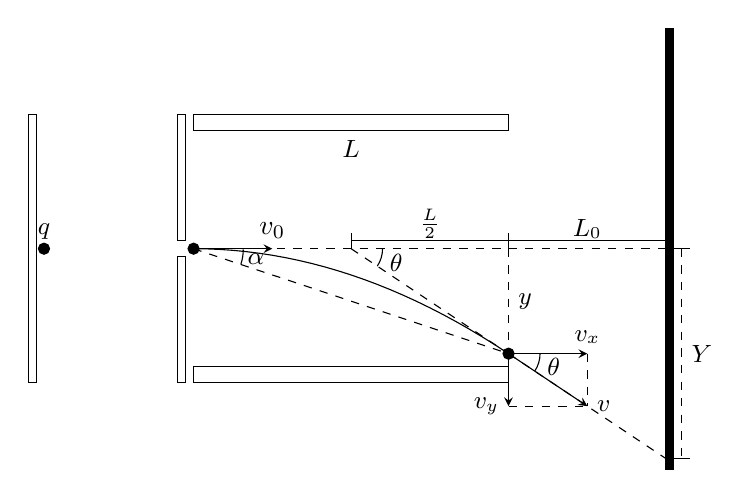
\begin{tikzpicture}
    \draw (-2,-1.7) rectangle (2,-1.5); 
    \draw (-2,1.7) rectangle (2,1.5); 
    \draw[dashed] (-2,0)--(2,0);
    \draw[domain=-2:2] plot (\x,-\x*\x/12-\x/3-1/3);
    \draw[->,>=stealth] (-2,0)--(-1,0) node [anchor=south]{$v_0$};
    \filldraw (-2,0) circle [radius=2pt];
    \draw[dashed](0,0)--(2,-1.333);
    \filldraw (2,-1.333) circle [radius=2pt];
    \draw[->,>=stealth] (2,-1.333)--++(1,-0.666) node [anchor=west]{\small $v$};
    \draw[->,>=stealth] (2,-1.333)--++(1,0) node [anchor=south]{\small $v_x$};
    \draw[->,>=stealth] (2,-1.333)--++(0,-0.666) node [anchor=east]{\small $v_y$};
    \draw[dashed](2,-1.333)++(1,0)--++(0,-0.666);
    \draw[dashed](2,-1.333)++(0,-0.666)--++(1,0);
    \draw[dashed](-2,0)--(2,-1.333);
    \draw (-2,0)++(0.6,-0.1998) arc (-18.433:0:0.6);
    \draw (-2,0)++(-9.22:0.8) node {\small $\alpha$};
    \draw(2,-1.333)++(-33.6874:0.4) arc (-33.6874:0:0.4);
    \draw(0,0)++(-33.6874:0.4) arc (-33.6874:0:0.4);
    \draw(2,-1.333)++(-16.8437:0.6) node {\small $\theta$}; 
    \draw(0,0)++(-16.8437:0.6) node {\small $\theta$}; 
    \draw (0,1.5) node [anchor=north]{\small $L$};
    \draw[dashed](2,0)--(2,-1.333);
    \draw (2,-0.666) node [anchor=west] {\small $y$};
    \draw (-2.1,-1.7) rectangle (-2.2,-0.1);
    \draw (-2.1,1.7) rectangle (-2.2,0.1);
    \draw (-4.1,-1.7) rectangle (-4,1.7);
    \filldraw (-3.9,0) circle [radius=2pt] node [anchor=south]{\small $q$};
    \filldraw (4,-2.8) rectangle (4.1,2.8);
    \draw[dashed] (2,-1.333)--(4,-2.666);
    \draw[dashed] (2,0)--(4,0);
    \draw (2,0)--(2,0.2);
    \draw (2,0.1)--(4,0.1);
    \draw (3,0) node [anchor=south]{\small $L_0$};
    \draw (0,0)--(0,0.2);
    \draw (0,0.1)--(2,0.1);
    \draw (1,0) node [anchor=south] {\small $\frac{L}{2}$};
    \draw (4.1,0)--(4.3,0);
    \draw (4.1,-2.666)--(4.3,-2.666);
    \draw[dashed] (4.2,0)--(4.2,-2.666);
    \draw (4.2,-1.333) node [anchor=west]{\small $Y$};
  \end{tikzpicture}
  \caption{屏幕上的偏移量}
  \label{fig:ddlzjspzpm}
\end{figure}

由几何关系很容易得出这个屏幕上的偏移量为
\begin{gather}
Y=(\frac{L}{2}+L)_0)\tan\theta=(\frac{L}{2}+L_0)\cdot\frac{U_2}{U_1}\cdot\frac{L}{2d}
\end{gather}
